\chapter{Présentation de l'entreprise d'accueil - SEBN-MA}
\label{chap:presentation_entreprise}

\section*{Introduction}
\addcontentsline{toc}{section}{Introduction}
Dans ce chapitre, je commencerai par une présentation de l'entreprise d'accueil, de sa structure intérieure, de ses clients et de ses réalisations. Une deuxième partie de ce chapitre concerne une analyse détaillée du cycle de production de l'usine, en mettant l'accent sur les différentes étapes et les technologies utilisées pour optimiser l'efficacité et la qualité de la production.

% ---------------------------------------------------------
\section{Présentation générale de l'entreprise}

\subsection{Nom et identité juridique}
L'entreprise d'accueil se nomme \textbf{SUMITOMO ELECTRIC BORDNETZE Morocco (SEBN-MA)}. Il s'agit d'une Société à Responsabilité Limitée à Associé Unique (SARL AU), filiale du groupe japonais Sumitomo Wiring Systems (SWS), dont le capital social s'élève à 140 000 000 d'euros.

Créée en 2001, SEBN-MA est spécialisée dans la conception et la fabrication de faisceaux électriques destinés à l'industrie automobile. Grâce à son expertise et à son savoir-faire, l'entreprise fournit plusieurs grands constructeurs automobiles internationaux et contribue au développement du secteur automobile au Maroc.

Mon stage s'est déroulé sur le site de Tanger, où sont réalisées les différentes opérations de production, d'assemblage et de contrôle des faisceaux électriques.

\subsection{Secteur d'activité}
SEBN opère dans le secteur du câblage automobile, en tant que fournisseur de Rang 1 (Tier 1). Cela signifie que l'entreprise livre directement les KSK, Autarkies, Batteries \& HV, sans intermédiaire. Le groupe est certifié selon les normes IATF 16949 (management de la qualité dans l'automobile), ISO 9001 et ISO 14001 (management environnemental), ISO 45001:2018 (management de la santé et de la sécurité au travail).

\subsection{Localisation}
SE Bordnetze Morocco (SEBN-MA) dispose de plusieurs sites de production au Maroc, notamment à Tanger Free Zone (TFZ), Tanger Automotive City (TAC) et Bouknadel (Salé).

Le site de Tanger Free Zone, où s'est déroulé mon stage, est implanté dans la région de Tanger-Tétouan-Al Hoceïma. Grâce à cette localisation stratégique et à la complémentarité de ses différents sites industriels, SEBN-MA assure efficacement la production et l'approvisionnement de nombreux constructeurs automobiles européens, tout en répondant aux exigences de qualité, de coût et de délai de ses clients.

Bien que les trois sites exercent la même activité principale, à savoir la fabrication de faisceaux électriques destinés à l'industrie automobile, le présent rapport porte exclusivement sur le site de Tanger Free Zone (TFZ).

\begin{figure}[H]
    \centering
    % Remplace 'nom_de_l_image.png' par ton fichier
    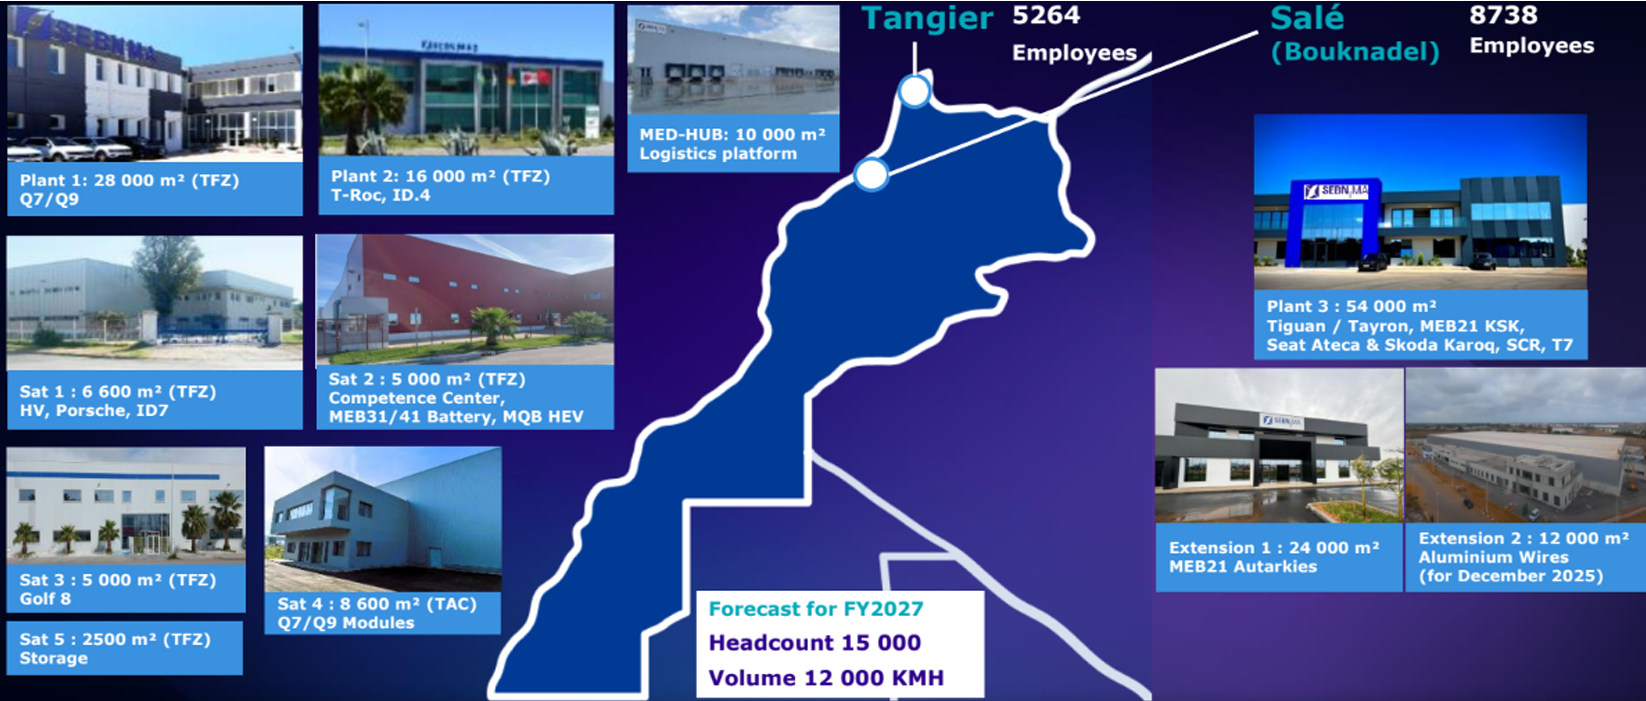
\includegraphics[width=0.7\textwidth]{images/Ch1/01.png} 
    \caption{Zone géographique de SEBN-MA} 
    \label{fig:zone_geo_sebn}
\end{figure}

\subsection{Certifications et achèvements}
SEBN-MA accorde une grande importance à la qualité, à la sécurité et à l'amélioration continue de ses processus. Grâce à son engagement envers les normes internationales et les exigences de ses clients, l'entreprise a obtenu plusieurs certifications, notamment IATF 16949, ISO 14001 et ISO 45001. Elle a également reçu plusieurs distinctions décernées par des constructeurs automobiles tels qu'Audi, SEAT et Volkswagen, témoignant de la fiabilité de ses produits et de la performance de son système de management.
\begin{figure}[H]
    \centering
    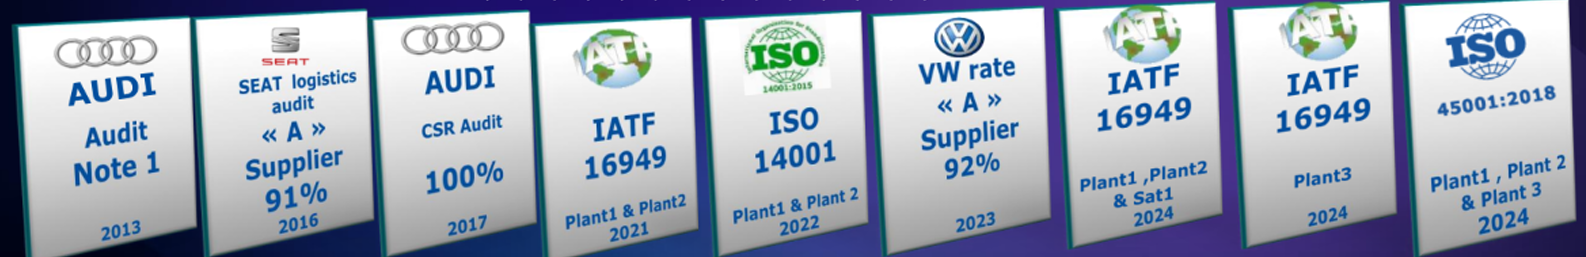
\includegraphics[width=0.7\textwidth]{images/Ch1/02.png} 
    \caption{Certifications et distinctions de SEBN-MA} 
    \label{fig:certifications_sebn}
\end{figure}

\subsection{Fiche signalétique}

% Réactivation des couleurs alternées pour ce tableau (si désactivé)
\rowcolors{2}{rowlight}{white}

\begin{table}[H]
    \centering
    \caption{Informations générales de SEBN-MA}
    \label{tab:fiche_signaletique}
    \vspace{0.3cm} % Petit espace entre le titre et le tableau
    
    % On utilise tabularx pour que le tableau prenne toute la largeur
    % La première colonne (Élément) fait 4.5cm et est en gras
    % La deuxième (Information) s'adapte automatiquement avec 'X'
    \begin{tabularx}{\textwidth}{>{\bfseries}p{4.5cm} X}
        \toprule
        % En-tête coloré
        \rowcolor{headerblue}
        \textcolor{white}{\textbf{Élément}} & \textcolor{white}{\textbf{Information}} \\
        \midrule
        
        Raison sociale    & SE Bordnetze Morocco (SEBN-MA) \\
        Forme juridique   & Société à Responsabilité Limitée à Associé Unique (SARL AU) \\
        Date de création  & 2001 \\
        Capital social    & 140 000 000 \texteuro \\ % ou "euros"
        Siège social      & Tanger Free Zone, Maroc \\
        Activité          & Fabrication de faisceaux électriques automobiles \\
        Groupe            & Sumitomo Wiring Systems (SWS) \\
        Certifications    & IATF 16949, ISO 9001, ISO 14001, ISO 45001:2018 \\
        
        \bottomrule
    \end{tabularx}
\end{table}
% ---------------------------------------------------------
\section{Historique et évolution du groupe}

\subsection{Origines}
La famille Sumitomo trouve ses origines au Japon au début du 17\up{e} siècle. Elle a été fondée par Masatomo Sumitomo, un marchand visionnaire qui a établi les bases solides de l'entreprise familiale. L'origine de la famille Sumitomo remonte aux débuts de Sumitomo House, qui a prospéré grâce au commerce du cuivre et d'autres marchandises. 

Masatomo Sumitomo a laissé derrière lui les "Préceptes du Fondateur", un ensemble de principes qui ont façonné la philosophie de Sumitomo en matière de conduite commerciale. Ces préceptes ont guidé la famille Sumitomo à travers les générations, contribuant à son succès durable et à sa réputation d'intégrité et d'engagement envers la communauté et le développement économique. Aujourd'hui, la famille Sumitomo est à la tête d'un vaste groupe d'entreprises diversifiées opérant dans différents secteurs à travers le monde.

% Affichage de deux images côte à côte pour gagner de la place et faire plus professionnel
\begin{figure}[H]
    \centering
    \begin{minipage}{0.45\textwidth}
        \centering
        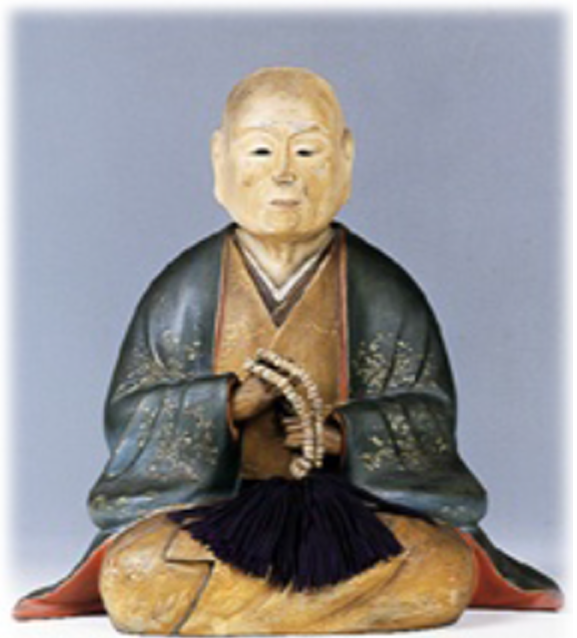
\includegraphics[width=0.9\linewidth]{images/Ch1/03.png}
        \caption{Statue en bois de Masatomo Sumitomo}
        \label{fig:statue_sumitomo}
    \end{minipage}\hfill
    \begin{minipage}{0.45\textwidth}
        \centering
        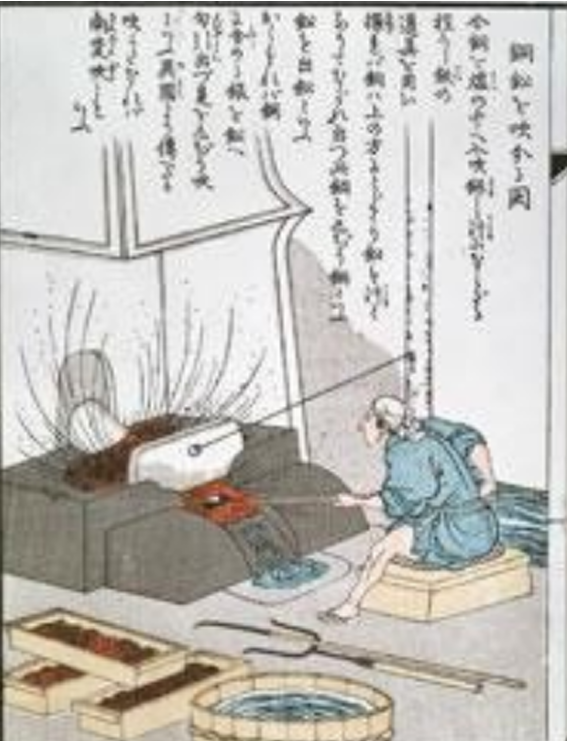
\includegraphics[width=0.9\linewidth]{images/Ch1/04.png}
        \caption{Méthode originale d'affinage du cuivre (Sumitomo Group)}
        \label{fig:affinage_cuivre}
    \end{minipage}
\end{figure}

\subsection{Le groupe Sumitomo Electric Bordnetze}
Le groupe SUMITOMO ELECTRIC BORDNETZE est un équipementier automobile spécialisé dans la fabrication des faisceaux électriques automobiles. Il a vu sa naissance pour la première fois en 1986 en tant qu'une joint-venture entre le groupe VOLKSWAGEN AG et SIEMENS AG. En effet, le groupe a été nommé pour la première fois VOLKSWAGEN BORDNETZE GMBH, alors qu'en 2006, il a poursuivi son activité sous le nom SUMITOMO ELECTRIC BORDNETZE après son rachat par le fameux groupe japonais SUMITOMO ELECTRIC INDUSTRIES.

Le groupe possède 39 sites implantés dans 13 pays, avec un siège central installé à Wolfsburg en Allemagne. De plus, le groupe emploie près de 39 000 employés de différentes nationalités.

\begin{figure}[H]
    \centering
    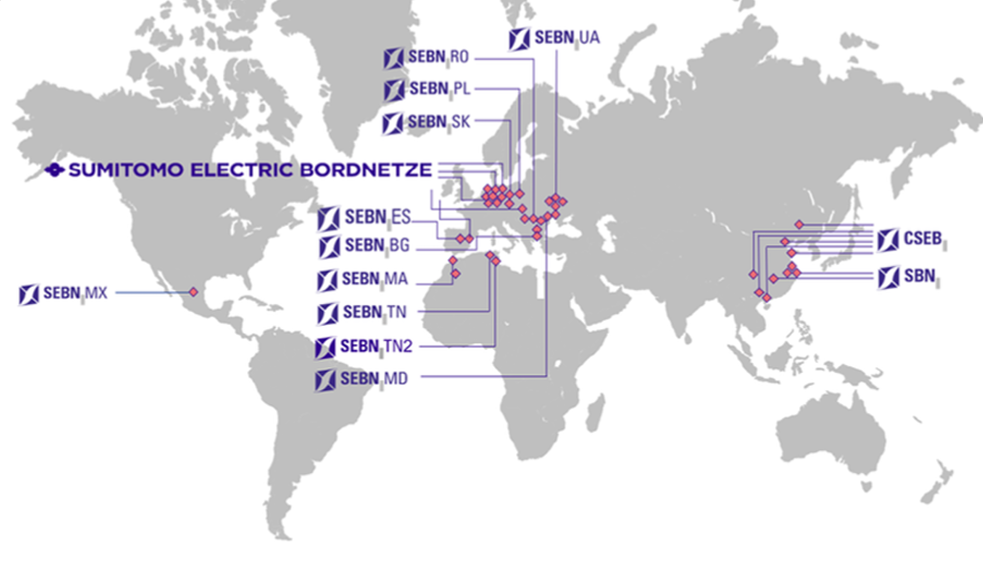
\includegraphics[width=0.8\textwidth]{images/Ch1/05.png}
    \caption{Les sites de SUMITOMO ELECTRIC BORDNETZE}
    \label{fig:sites_sebn}
\end{figure}

\subsection{L'historique de SEBN-MA}

\begin{figure}[H]
    \centering
    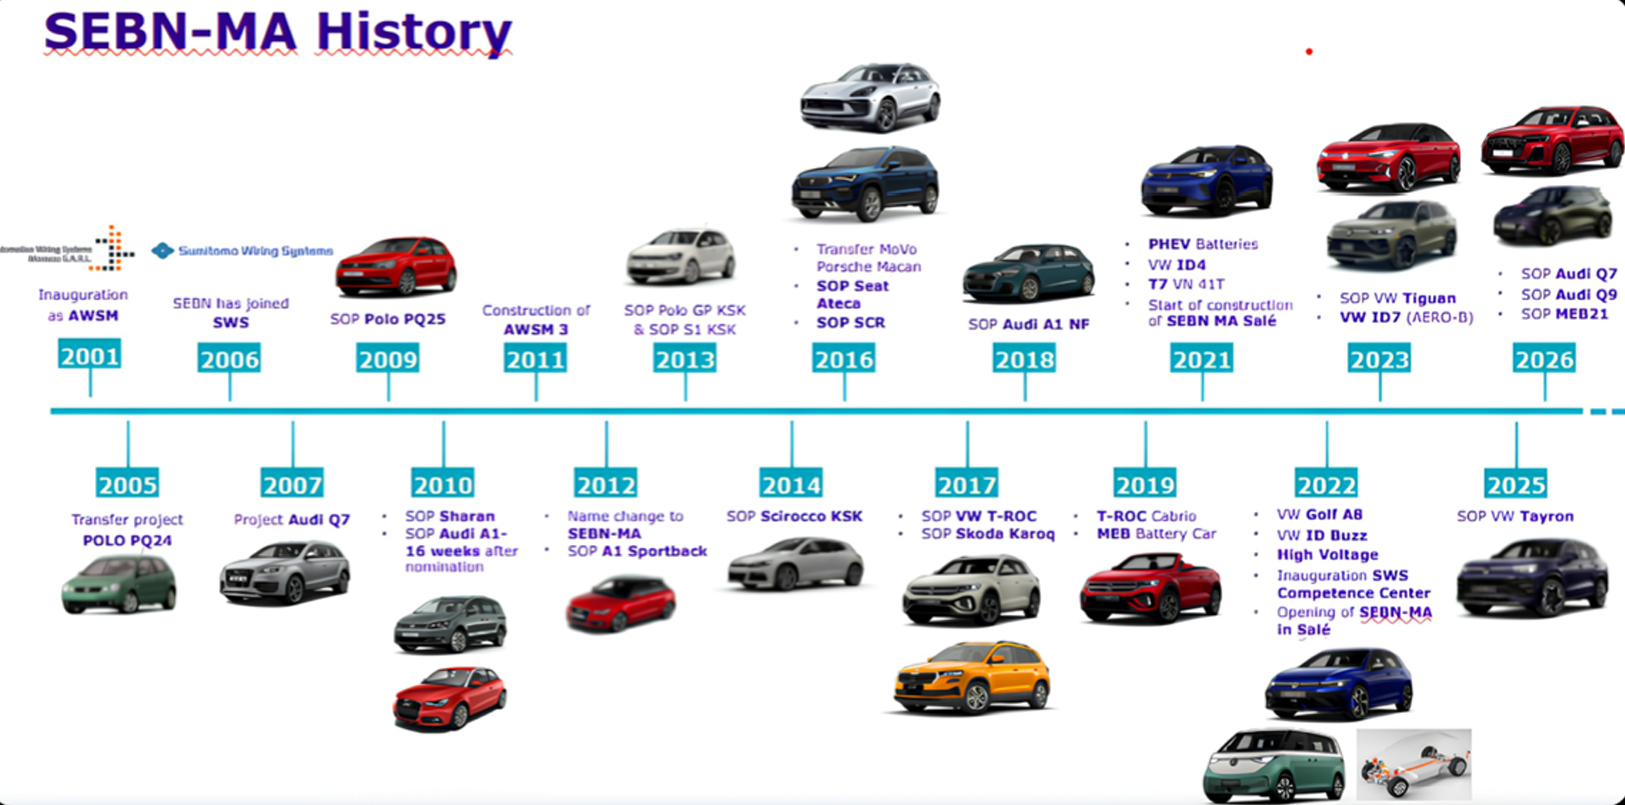
\includegraphics[width=0.85\textwidth]{images/Ch1/06.png}
    \caption{Historique de SEBN-MA}
    \label{fig:historique_sebn_ma}
\end{figure}


% ---------------------------------------------------------
\section{Activités et domaines d'intervention}

\subsection{Les différents câbles produits par SEBN-MA}
Au sein de SEBN-MA se fait la production de deux types de câbles. On trouve :

\begin{itemize}
    \item \textbf{Projet KSK :} C'est un ensemble des faisceaux de câbles électriques rassemblés dans un seul câble qui sera lié directement au moteur et qui contient essentiellement les câbles de base comme celui du frein, des feux, etc., plus les spécifications des clients. C'est le câble principal de la voiture.
    \begin{itemize}
        \item \textit{KSK INRA :} Partie compartiment.
        \item \textit{KSK MORA :} Partie moteur.
    \end{itemize}
    
    \item \textbf{Les projets Autarks :} Ce sont des faisceaux de câbles des équipements et des options de voitures telles que les portières, les vitres, les sièges, l'Airbag...
\end{itemize}

\begin{figure}[H]
    \centering
    \begin{minipage}{0.45\textwidth}
        \centering
        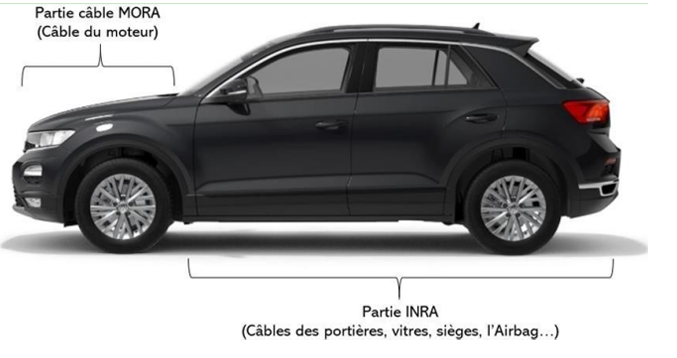
\includegraphics[width=0.9\linewidth]{images/Ch1/07.png}
        \caption{Partie câble MORA et INRA de voiture T-ROC}
        \label{fig:cable_mora_inra}
    \end{minipage}\hfill
    \begin{minipage}{0.45\textwidth}
        \centering
        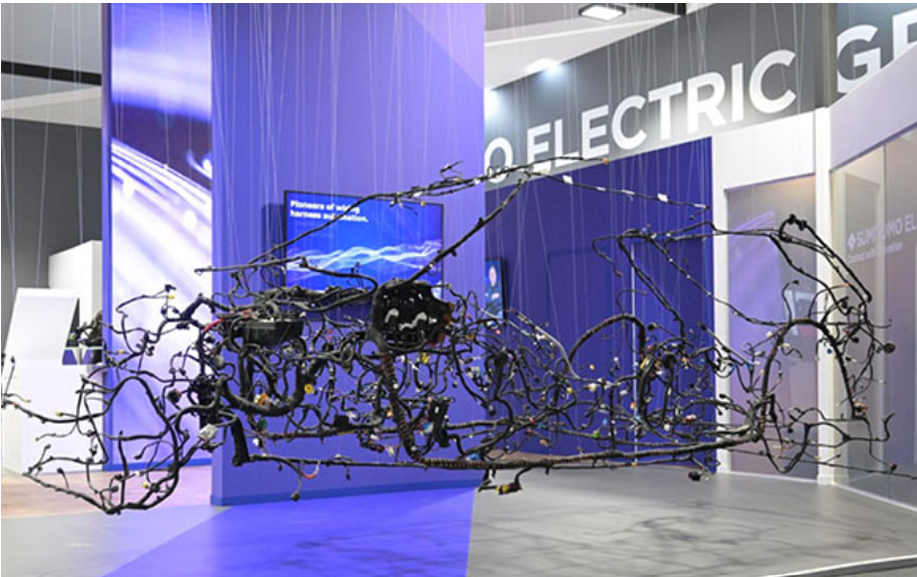
\includegraphics[width=0.9\linewidth]{images/Ch1/08.png}
        \caption{Exemple d'un faisceau électrique (KSK)}
        \label{fig:faisceau_ksk}
    \end{minipage}
\end{figure}

\subsection{Produits et Clients de SEBN-MA}
SE Bordnetze Morocco (SEBN-MA) est spécialisée dans la fabrication de faisceaux électriques destinés à l'industrie automobile. La filiale marocaine produit principalement trois familles de produits : les faisceaux électriques conventionnels (KSK), les systèmes électriques autonomes (Autarkies) ainsi que les faisceaux destinés aux véhicules électriques et hybrides, notamment les systèmes High Voltage (HV) et les ensembles de batteries.

\begin{figure}[H]
    \centering
    \begin{minipage}{0.45\textwidth}
        \centering
        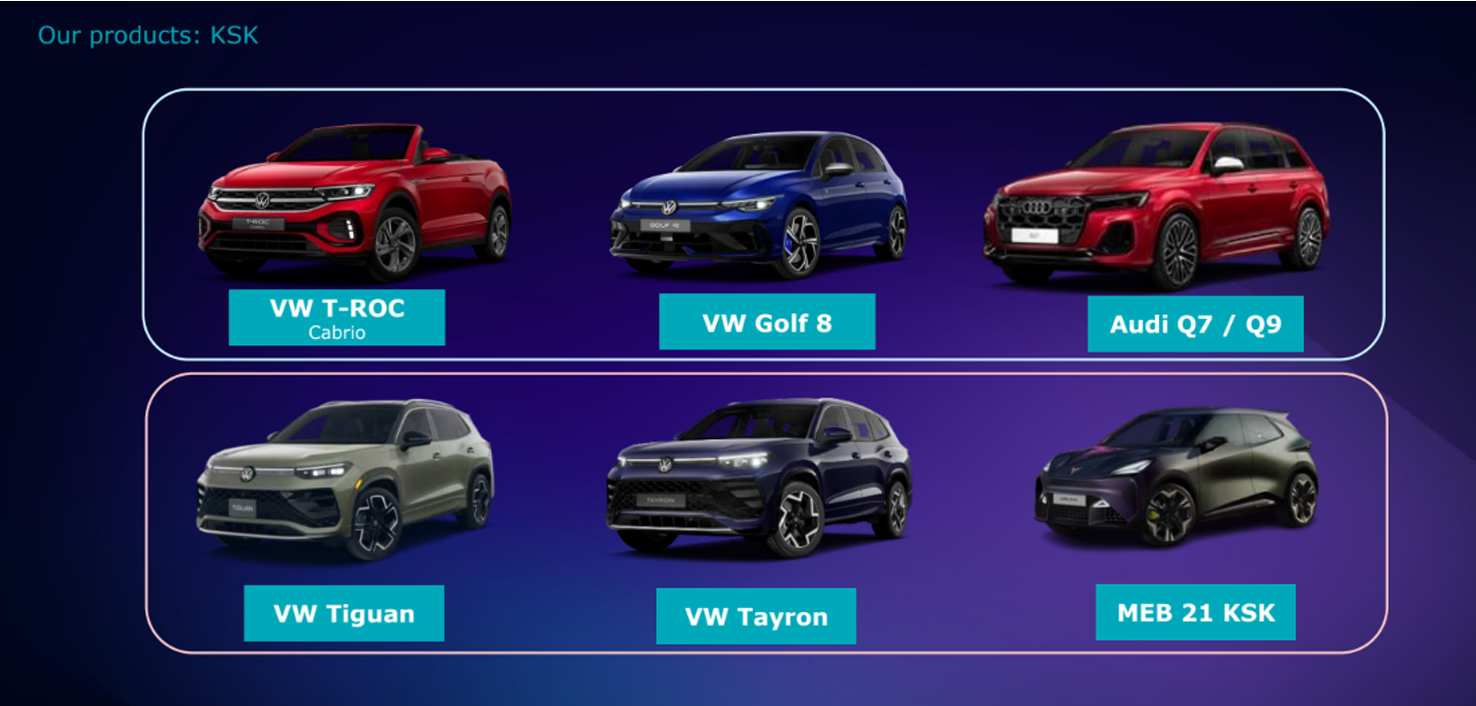
\includegraphics[width=0.9\linewidth]{images/Ch1/09.png}
        \caption{Les produits de KSK}
        \label{fig:produits_ksk}
    \end{minipage}\hfill
    \begin{minipage}{0.45\textwidth}
        \centering
        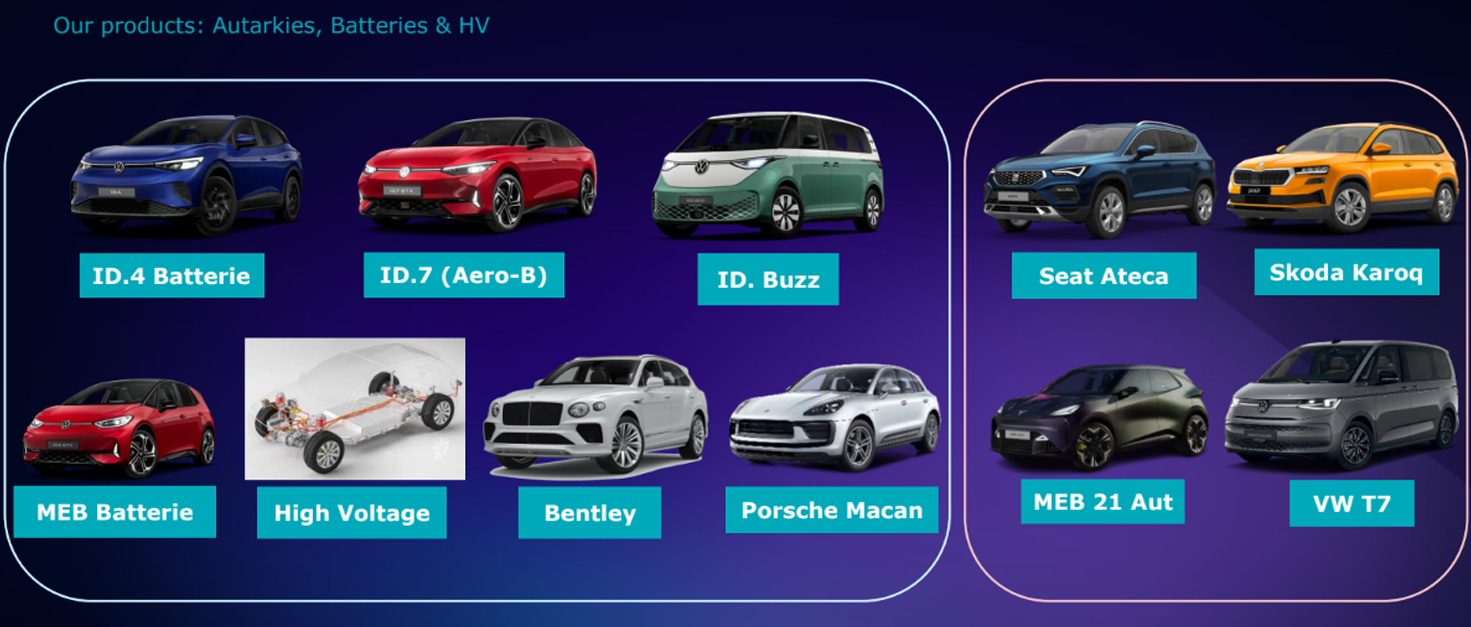
\includegraphics[width=0.9\linewidth]{images/Ch1/10.png}
        \caption{Les produits Autarkies, Batteries \& HV}
        \label{fig:produits_autarkies}
    \end{minipage}
\end{figure}

SEBN-MA est un fournisseur de premier rang (Tier 1) de l'industrie automobile, collaborant avec plusieurs constructeurs automobiles de renommée mondiale. Parmi ses principaux clients figurent les marques du groupe Volkswagen, telles que Volkswagen, Audi, Škoda, SEAT, CUPRA, Porsche et Bentley. Grâce à ses sites de production implantés au Maroc, l'entreprise assure l'approvisionnement des usines de ses clients situées principalement en Allemagne, en Espagne, en Slovaquie, en République tchèque et au Royaume-Uni, tout en garantissant des produits conformes aux exigences de qualité, de coût et de délai.

% ---------------------------------------------------------
% Note : LaTeX gérera automatiquement la numérotation. 
% Même si tu as écrit 1.5 dans ton brouillon, LaTeX l'affichera comme 1.4 car c'est la 4ème section.
\section{Organisation de l'entreprise}

\subsection{Principaux départements et leurs rôles}
L'efficacité industrielle du site repose sur une organisation fonctionnelle où chaque département contribue spécifiquement à la performance globale. Les principaux services et leurs missions sont décrits ci-après :

\begin{itemize}
    \item \textbf{Département Ressources Humaines (PHR) :} Le département RH a une double mission : il assure d'une part la gestion du volet administratif du personnel (la paie, les prestations sociales) et d'autre part la gestion de l'absentéisme et de la discipline.
    
    \item \textbf{Département Finance (PCP) :} Ce département a pour mission de gérer toutes les opérations de comptabilité et de trésorerie tout en restant en contact permanent avec les clients, les fournisseurs et les différents acteurs internes et externes à l'entreprise.
    
    \item \textbf{Département Controlling (PMC) :} Il coordonne, évalue et surveille toutes les activités liées au contrôle de gestion ainsi qu'aux opérations de suivi du budget.
    
    \item \textbf{Département Projet (PPM) :} Le département PO définit et maintient le référentiel des processus liés à la gestion de projet.
    
    \item \textbf{Département Technique (PTS) :} La principale mission de ce département (OHS-Environnement) est d'assurer l'application et la diffusion des règles de sécurité de l'entreprise en informant les employés sur les mesures de prévention. Il analyse les incidents afin d'en déterminer les causes et en déduit des actions d'amélioration et de prévention des risques.
    
    \item \textbf{Département Informatique (PIT) :} Chargé de l'administration du système d'information, le département informatique s'occupe de la gestion du parc informatique, incluant l'installation et l'entretien du réseau et des serveurs. En outre, ce service est chargé de gérer les applications et les ERP des différents départements.
    
    \item \textbf{Département Ingénierie (PPE) :} Ce département est chargé d'optimiser la planification de la production en fonction des besoins des clients et des objectifs internes. \textit{C'est le département dans lequel j'ai effectué mon stage.}
    
    \item \textbf{Département Production (PPR) :} La mission principale de ce département est d'assurer l'exécution de la production selon les normes des clients (fournies par le département planning) et selon les exigences des normes de qualité (normes client et normes IATF 16949).
    
    \item \textbf{Département Logistique (PLM) :} La fonction logistique a pour objectif de veiller à l'harmonie totale et à la parfaite synchronisation entre les flux de matières et les flux d'informations (production en Juste-à-Temps). Le département assure aussi l'approvisionnement, la gestion des stocks, l'ordonnancement de la production, le transport, etc.
\end{itemize}